\documentclass[a4paper,12pt]{article}

% Packages
\usepackage{graphicx} % For including images
\usepackage{titlesec}
\usepackage{titling}
\usepackage{setspace}
\usepackage{fancyhdr}
\usepackage{geometry}
\geometry{margin=1in}
\usepackage{xcolor} % For colours %%\textcolor{red}{This is red text.} \textcolor{blue}{Important term}
\usepackage{soul} % For highlights  %%\hl{This is highlighted text.}
\usepackage{amsmath}  % For math symbols
\usepackage{amssymb}  % For additional symbols
\usepackage[utf8]{inputenc} % For handling special characters

% Title and Author
%\title{Classical Mechanics}
%\author{Joshua Quaye\thanks{CLASSICAL MECHANICS I. PHY. 253}}

\begin{document}
\begin{center}
\textbf{\Large{KWAME NKRUMAH UNIVERSITY OF SCIENCE}} \\
\vspace{0.4cm}
\textbf{\Large{AND TECHNOLOGY}} \\
\rule{\linewidth}{0.4pt} % Horizontal line
\end{center}

\vspace{1.5cm}

% Course Title
\begin{center}
\textbf{\LARGE{CLASSICAL MECHANICS I}} \\
\rule{0.6\linewidth}{0.4pt}
\end{center}

\vspace{1.5cm}

% University Logo
\begin{center}

\includegraphics[width=0.3\textwidth]{logo.jpg}
\end{center}
\rule{\linewidth}{0.3pt}

\vspace{1.5cm}

% Department Info
\begin{center}
\large{\textbf{\textit{
Department Of Physics \\
Faculty Of Physical and Computational Sciences \\
College Of Science \\
Kwame Nkrumah University of Science and Technology
}}}
\end{center}


%\vspace{3cm}


%\maketitle
\begin{thanks}
CLASSICAL MECHANICS I. PHY. 253
\end{thanks}
\newpage



%\begin{frame}{GROUP MEMBERS}
\begin{center}
\Large{\textbf{\underline{GROUP MEMBERS}}}\\
\vspace{1cm}
\\
 \begin{tabular}{ll}
 \LARGE{
\textbf{Name}                  &\textbf{Index Number}\\
\textbf{ Arhin Joshua Quaye}            &\textbf{9130223}\\
Abena Konadu Asubonteng        &8665421\\ 
Kelly Nyarko                   &8656521\\
Edna kamasin                   &8664421\\
Atsutse Nelly                  &8664221\\
Baidoo Ruth                    &8667121\\
Opare Boakye Joshua            &8665621\\
Samuel                         &8661721\\
Gyimah Benjamin                &4279120\\
Danso Afrifa Eric              &8661321\\
Michael Okyere                 &8664821\\
%\end{tabular}
\end{center}}

%\end{frame}}
\newpage
\tableofcontents

\section{Introduction}
% Add your introduction content here
Introduction to Classical Mechanics

Galileo first laid down the fundamental principles of classical mechanics and followed Newton’s work. Classical mechanics is the study of the motion of bodies (including the special case in which bodies remain at rest according to the general principles of first
enunciated by Sir Isaac Newton in his famous book Philosophiae Naturalis Principia Mathematica
(1687), commonly referred to as the Principia. Newton propounded three laws of motion, and one law
of gravity and pretended he did not know calculus. Probably the single greatest scientific achievement in history, you might think this pretty much wraps it up for classical mechanics. And in a
sense, it does.
Classical mechanics was the first branch of Physics to be discovered and is the basis upon
which all other branches of Physics depend. Classical mechanics has many important applications
in other areas of science, such as Astronomy (celestian mechanics), Chemistry (the dynamics of
molecular collisions) Geology (the propagation of of seismic waves, generated by earthquakes,
through the Earth’s crust) and Engineering (the equilibrium and stability of structures). Classical
mechanics is also of great significance outside the realm of science. After all, the sequence of
events leading to the discovery of classical mechanics-starting with the ground-breaking work of
Copernicus, continued with the research of Galileo, Keppler, Descartes and culminating in the
monumental achievement of Newton-involved the complete overthrow of the Aristotelian picture
of the Universe, which had previously prevailed for more than a milennium, and its replacement
by a recognizably modern picture in which humankind no longer played a privileged role.
Given a collection of particles, acted upon by a collection of forces, you have to draw a nice
diagram, with the particles as points and the forces as arrows. The forces are then added up and
Newton’s famous ”F = ma” is employed to figure out where the particles velocities are heading
next. All you need is enough patience and a big computer and you are done.
From a modern perspective, this is a little unsatisfactory on several levels: It’s messy and inelegant; it is hard to deal with problems that involve extended objects rather than points particles; it
obscures certain features of dynamics so that concepts such as chaos theory took over 200 years to
discover; and its not all clear what the relationship is between Newton’s classical laws and quatum
physics.
Classical mechanics covers the following: 
\begin{itemize}
    \item The case in which bodies remain at rest.
    \item Translational motion: by which a body shifts from one point in space to another.
    \item Oscillatory motion: example; the motion of a pendulum or spring.
    \item Circular motion: example; the motion of the earth around the sun.
    \item More general rotational motion: orbits of the planets or bodies that are spinning.
    \item Particle collisions (elastic and inelastic).
    
\textitalic{It is also concerned with:}
    \item Motion of objects: velocity and acceleration.
    \item Causes of the motion: force and energy.
    \item Newton’s three laws of motion.
\end{itemize}

\subsection{Application of Classical Mechanics in areas of science}

\begin{enumerate}
    \item \textbf{Astronomy:} How planets move around the sun, motion of stars.
    \item \textbf{Molecular and Nuclear Physics:} Collision of atomic and subatomic particles, how an electron moves around the nucleus of an atom.
    \item \textbf{Geology:} The propagation of seismic waves.
    \item \textbf{Engineering:} Structure of bridges and buildings, how a skier moves down the slope.
\end{enumerate}

\newpage
\section{Space and Time}
Newton’s three laws are formulated in terms of four crucial underlying concepts: the motion of
 space, time, mass and force.
\subsection{Space}
% Add content extracted from your PDF here
Each point \textbf{P} of three-dimensional space in which we live can be labelled by a position vector r which specifies the distance and direction of \textbf{P} from a chosen origin \textbf{O}, as seen in figure 1.
\begin{figure}[h] % "h" means place it 'here'
    \centering
    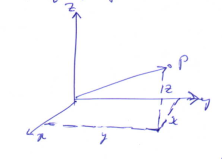
\includegraphics[width=0.7\textwidth]{space.png}
    \caption{space coordinate}
    \label{figure 1}
\end{figure}

There are many different ways to identify a vector. The most natural way to identify a vector is to give its components \((x, y, z)\) in the direction of three chosen perpendicular axes. One particular way to express this is to introduce three unit vectors \( \[\hat{x},\ \hat{y},\ \hat{z},\ \]\) pointing along the three axes and to write \(\[\vec{r} = x \, \hat{x} + y \, \hat{y} + z \, \hat{z}\]\).
Our popular choice is to use \( i, j, k \) for \( \hat{x}, \hat{y}, \hat{z} \):
\[\vec{r} = (x, y, z) = (r_1,\ r_2,\ r_3) = (e_1,\ e_2,\ e_3)\]
\[r_1 = x, \quad r_2 = y, \quad r_3 = z\]
\[e_1 = \hat{x}, \quad e_2 = \hat{y}, \quad e_3 = \hat{z}\]
The symbol \( e \) is commonly used for unit vectors. Since \( e \) stands for the German word "eins" or "one":
\[\vec{r} = r_1 e_1 + r_2 e_2 + r_3 e_3 = \sum_{i=1}^{3} r_i e_i\]
%\[r_i e_i\]


\subsection{Vector operations}
% Add content extracted from your PDF here
In our study of mechanics, we shall make repeated use of the various operations that can be performed with vectors. If r and s are vectors with the components \(\[\vec{r} = (r_1,\ r_2 ,\ r_3 )\]\) and \(\[\vec{s} =
(s_1,\ s_2 ,\ s_3 )\]\), their sum is by adding corresponding components. Thus,
\[\vec{r} + \vec{s} = (r_1\ +\ s_1 ,\  \ \ r_2\ +\ s_2 ,\ \ r_3 + s_3)\]
An important example of a vector is the resultant force on an object.
When two forces Fa and Fb act on an object, the effect is the same as single force. The resultant
force, which is just the vector sum \(\[F = F_a + F_b\]\) . if c is a scalar and $\[\vec{r}\] is a vector, the product c$\[\vec{r}\] is
given by:
\(c\[\vec{r} = (cr_1,\ cr_2 ,\ cr_3 )\]\)
This means c\(\[\cdot\]\)r is a vector in the same direction as r with magnitude equal to c times the magnitude
of r.

\begin{center}
\underline{\textcolor{blue}{\textbf{This is just a trial matrix}}}    
\end{center}

%%matrix
\[
\vec{A} \times \vec{B} =
\begin{vmatrix}
\hat{i} & \hat{j} & \hat{k} \\
A_x & A_y & A_z \\
B_x & B_y & B_z
\end{vmatrix}
\]


{\Large \textbf{Illustration 1}}\\
An object of mass m(a scalar) has an acceleration a (a vector), Newton’s second law asserts that
the resultant force F on the object will always equal the product  \(\[F = ma\]\). Two important pair of product of pair vectors; the scalar product (or dot product)
\[\vec{r} \cdot \vec{s} = |r| |s|\ cos \theta\]
\[= r_1 s_1 + r_2 s_2 + r_3 s_3\]
\[= \sum^{3} _{i = 1} r_n s_n

{\Large \textbf{Illustration 2}}

If a force F acts on an object that moves through a displacement d\(\[\vec{r}\]\), then the workdone by its force is
 the scalar product F · d\(\[\vec{r}\]\). The magnitude of a vector(length) r is denoted by \(\[|r|\]\). By Pythagoras
 theorem

 \[ |r| = \sqrt{r^2 _1 + r^2 _2 + r^2 _3}\]
 . The second product of two vectors r and s is the vector product (or cross product) which defines
 the product \(\[p = \vec{r} ×\vec{s}\]\)
 \[p_x = r_ys_z −r_zs_y\]
 \[p_y = r_zs_x −r_xs_z\]
 \[p_z = r_xs_y −r_ys_x\]
 \begin{center}
     or
 \end{center}
 
 \[\vec{r} \times \vec{s} = det
 \begin{vmatrix}
 \hat{x}  &  \hat{y} & \hat{z}\\
 r_x & r_y & r_z\\
 s_x &  s_y  & s_z
 \end{vmatrix}\]

 
 The vector product plays an important role in the discussion of rotational motion. For example, the tendency of a force F acting at a point r to cause a body to rotate about the origin is given by
 the torque of F about O depends on the vector product
\(\large \mathbf{r} = \vec{r} \times F \) .


%\begin{figure}[h!]
%    \centering
%    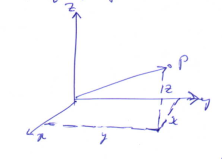
\includegraphics[width=\textwidth]{space.png} % Replace with the name of an actual image file
%    \caption{space coordinate}
%    \label{fig:label1}
%\end{figure}

\subsection{Vector Differenciation}

Many (maybe most) of the laws of physics involve vectors, and most of these involve derivatives
of vectors. For instance, the velocity of a particle is the time derivative of the particle’s position
r(t); that is \[V = \frac{d\vec{r}}{dt}\]
similarly, the acceleration \[a = \frac{dv}{dt}\]
We define derivative as \[\frac{dx}{dt} = \lim_{\Delta t \to 0} \frac{\Delta x}{\Delta t}\] where \[\Delta x = x(t + \Delta z) - x(t)\]
\[\Delta x \to \text{change of x}\] 
\[\Delta t \to \text{change in time}\]
\[\Delta r = r (t + \Delta t)\ -\ r(t)\]
All vectors we shall encounter are differencials and hence you can take for granted the limit exists.

If \[r(t)\ \text{and}\ s(t)\] are two vectors that depend on t then the derivative of their sum is first what you
 would expect:
 \[\frac{d}{dt}(r+t) = \frac{dr}{dt} + \frac{ds}{dt}\]
  similarly, if r(t) is a vector and f(t) is a scaler, then the derivative of the product f(t)r(t) is given
 by \[\frac{d}{dt}(r + s) = f\frac{dr}{dt} + \frac{df}{dt}r\]

\subsection{Time}

The classical view is that time is a single universal parameter t on which all observers agree. That is, if all observers are eqipped with accurate clocks, all properly synchronized, then they will all agree on to the time at which at which any given event occured. This view is not exactly correct; According to the theory of relativity, two observers in relative motion do not agree on all times! Nevertheless, in the domain of classical mechanics, with all speed much less than the speed of light c, the differences among the measured times are entirely negligible and therefore adopt the classical assumption of a single universal time. Apart from the obvious ambiguity in the choice of origin of time(the time that we choose to label as t = 0), all observers agree on the times of all events.

\subsection{Reference Frames}

Every problem in classical mechanics involves a choice of a reference frame. That is, a choice of spatial origin and axes to label positions as in Figure 1 and a choice of temporal origin to measure times.
\\
\\
 The difference between two frames maybe quite minor. For instance, they may differ only in their choice of the origin of time – what one frame labels \[t = 0\], the other may label \[t′ = t_o \neq 0\]. Or the two frames may have the same origins of space and time, but have different orientations of the three spatial axes. By carefully choosing your reference frame, taking advantage of these different possibilities, you can sometimes simplify your work. A more important difference arises when two frames are in relative motion; that is; when one origin is moving relative to the other. 
 
 
 \\We shall find that later, not all such frames are physically equivalent. In certain special frames, called \textit{inertial frames}, the basic laws hold time in their standard, simple form(it is because one of these basic laws is Newton’s first law, the law of inertial, that these frames are called inertial). 
 
 
 \\If a second frame is accelerating or rotating relative to an inertial frame, then this second frame is noninertial, and the basic laws– in particular, Newton’s law do not hold in their standard form in this second frame. We shall find that the distinction between inertial and noninertial frames is central to our discussion of classical mechanics. It plays an even more explicit role in the theory of relativity
\subsection{Galilean Transformatin}
\begin{figure}[h] % "h" means place it 'here'
    \centering
    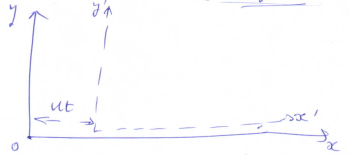
\includegraphics[width=0.7\textwidth]{Galilean.png}
    \caption{Galilean transformation}
    \label{figure 2}
\end{figure}


\[
\begin{array}{cc}
\text{S-frame} & \text{S'-frame} \\
x = x' + ut & x' = x - ut \\
y = y' & y' = y \\
z = z' & z' = z \\
\end{array}
\]
This coordinate of transformation was discovered by Galileo Galilei, hence they are called \textbf{Galilean transformation.}

Instantaneous velocity of an object in the first
\[v = \frac{dr}{dt}\]
\[V'_x = V_x - u\]
\[V'_y = V_y\]
\[V'_z = V_z\]
\[ V' = V - u\]
\[a = \frac{dv}{dt} = (\frac{dV_x}{dt}, \frac{dV_y}{dt}, \frac{dV_z}{dt})\]
\[a'_x = a_x\]
\[a'_y = a_y\]
\[a'_z = a_z\]
In a more compact form
\[a' = a\]
If an object is moving in a straight line with constant speed in our original inertial frame (ie y′ = 0), then it also moves in a (different) straight line with (a different) constant speed in the second frame of reference(i.e. a′ = 0). Hence, we conclude that the second frame of reference is also an initial frame. A simple extension of the above argument allows us to conclude that there are an
 infinit number of different inertial frames moving with constant velocities with respect to another.
 Newton thought one of these inertial frames was special, and defined an absolute standard of rest.
 i.e A static object in this frame was in a state of absolute rest. However, Einstein showed that this
 is not the case. In fact there is no absolute standard of rest, i.e, all motion is relative– hence, the
 name \textit{"relativity"} for Einstein theory. Consequently, one inertial frame is fast as another as far as
 Newtonian dynamics is concerned. But, what happens if the second frame of reference accelerates with respect to the first? In this
 case, it is not hard to see that (2.1) generalises to
 \[a' = a - \frac{du}{dt}\]
 where u(t) is the instantaneous velocity of the second frame with respect to the first. According
 to the above equation, if an object is moving in a straight–line with constant speed in the first
 frame(i.e a′ = 0), then it does not move in a straight–line with constant speed in the second frame
 (i.e \(a′\neq  0\)). Hence if the first frame is an inertial frame, then the second is not. A simple extention
 of the above argument allows us to conclude that any frame of reference which accelerates with respect to a given initial frame is not itself an inertial frame.
 For most practical purposes, when studing the motions of object close to the Earth’s surface, a
 reference frame which is fixed with respect to this surface is approximately inertial. Alternatively;
 If a second frame is accelerating or rotating relative to an inertial frame, then this second frame
 is noninertial, and the basic laws–Newton’s law do not hold in their standard form in the second
 frame.
 We shall find that, the distinction between inertial and noninertial frames is the central point of
 the discussion of classical mechanics.

 \newpage
 hiwiw
 
\end{document}
